\subsection{Phoneme decoding}
\label{sec:decoding}
In this section we quantify to what extent phoneme identity can be
decoded from  the input MFCC features as compared to the
representations extracted from the COCO speech. As explained in 
Section~\ref{sec:forced}, we use phonemic
transcriptions aligned to the corresponding audio in order to segment
 the signal into chunks corresponding to individual phonemes.

We take a sample of 5000 utterances from the validation set of
Synthetically Spoken COCO, and extract the force-aligned
representations from the Speech COCO model.
%using the procedure described in Section~\ref{sec:forced}. 
We split this data into $\frac{2}{3}$ training and
$\frac{1}{3}$ heldout portions, and use supervised classification in
order to quantify the recoverability of phoneme identities from the
representations. Each phoneme slice is averaged over time, so that it
becomes a $D_r$-dimensional vector. For each representation we then
train $L2$-penalized logistic regression (with the fixed penalty
weight $1.0$) on the training data and measure classification error rate
on the heldout portion. 

Figure~\ref{fig:decode} shows the results. As can be seen from this plot, phoneme recoverability 
is poor for the representations based on MFCC and the convolutional layer activations, but improves markedly for 
the recurrent layers. Phonemes are easiest recovered from the activations at recurrent
layers 1 and 2, and the accuracy decreases thereafter. This suggests
that the bottom recurrent layers of the model specialize in recognizing this
type of low-level phonological information. It is notable however that
even the last recurrent layer encodes phoneme identity to a
substantial degree.

The MFCC features do much better than majority baseline (89\% error rate) but
poorly relative to the the recurrent layers. Averaging across
phoneme durations may be hurting performance, but interestingly, the
network can overcome this and form more robust phoneme representations in 
the activation patterns.

\begin{figure}[t]
  \centering
  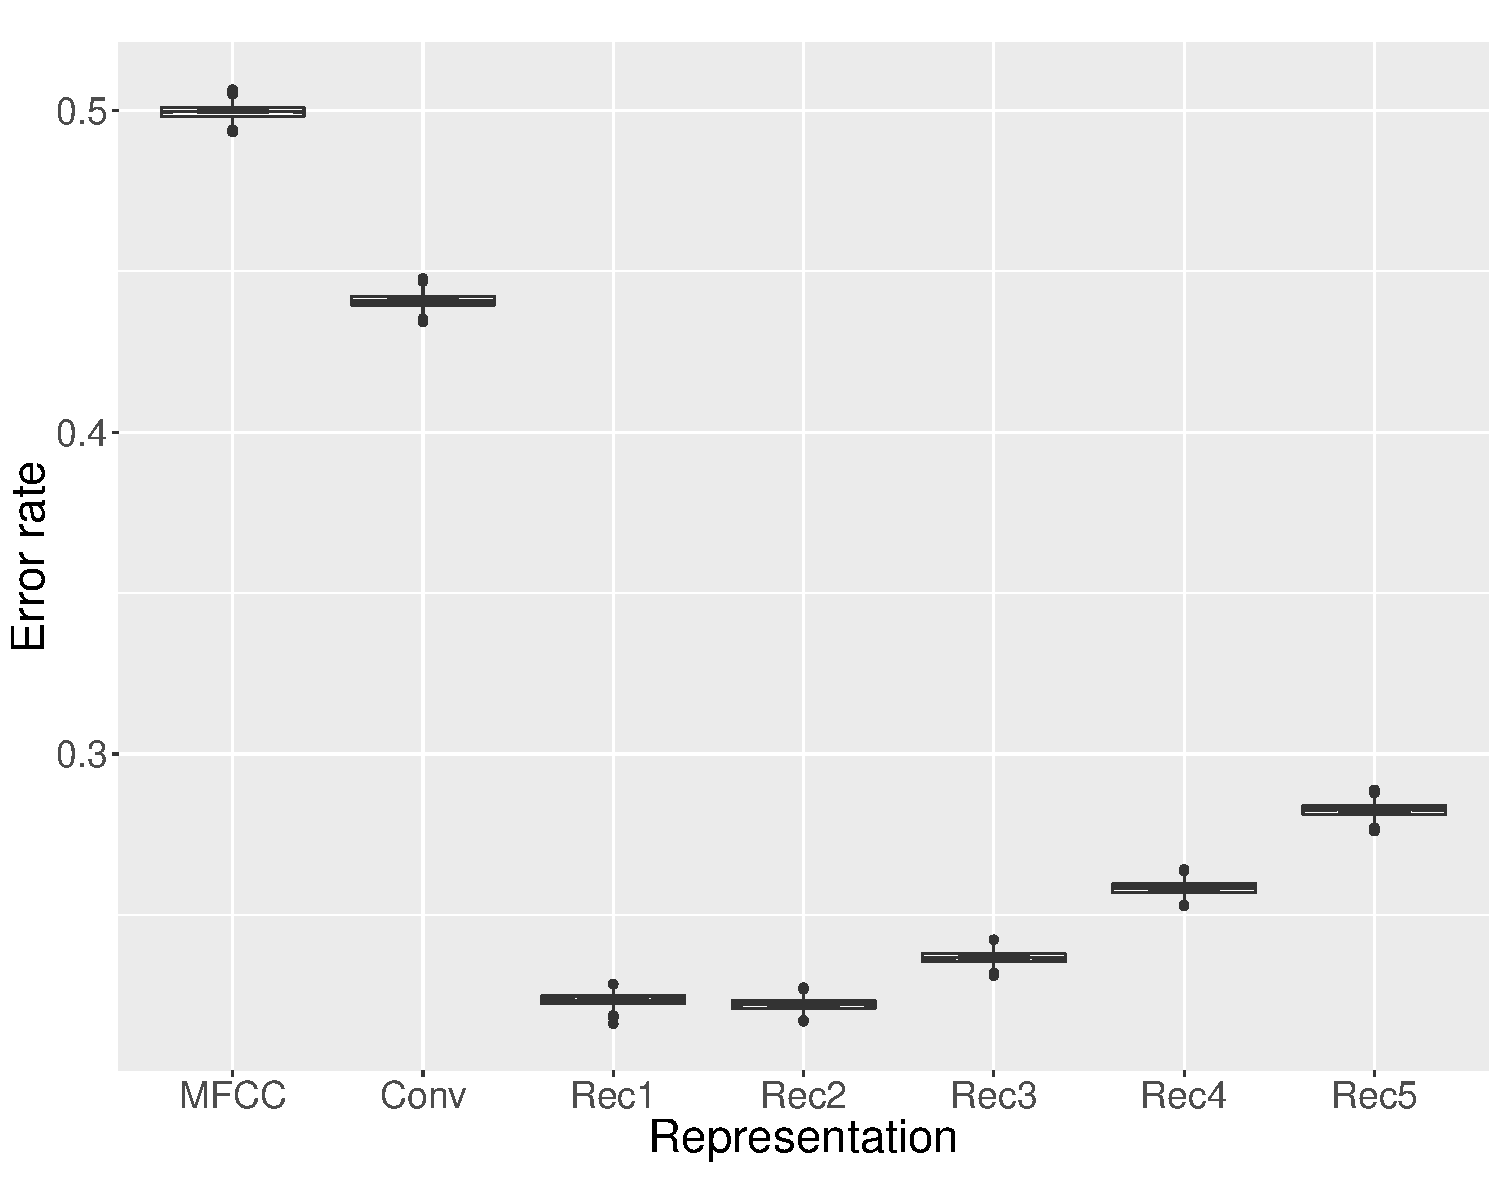
\includegraphics[scale=0.3]{figures/decode.pdf}
     \caption{Accuracy of phoneme decoding with input MFCC features
       and COCO~Speech model activations. The boxplot shows error rates
       bootstrapped with 1000 resamples.}
     \label{fig:decode}
\end{figure}
%% \begin{table}
%%   \centering
%%   \begin{tabular}{l|r}
%%     Representation  & Accuracy  \\\hline
%%     MFCC            & 0.50      \\\hdashline
%%     Convolution     & 0.56      \\
%%     Recurrent 1     & 0.77      \\
%%     Recurrent 2     & 0.78      \\
%%     Recurrent 3     & 0.76      \\
%%     Recurrent 4     & 0.74      \\
%%     Recurrent 5     & 0.72      \\
%%   \end{tabular}
%%   \caption{Accuracy of phoneme decoding with input MFCC features and
%%     COCO~Speech model activations.}
%%   \label{tab:decode}
%% \end{table}
%% ('mfcc', 0.49870657476692304)
%% ('conv', 0.55728398062466367)
%% (0, 0.77430163718120104)
%% (1, 0.77633292244657026)
%% (2, 0.76174933592597094)
%% (3, 0.74003020885779269)
%% (4, 0.71567214708588689)

